\documentclass[unknownkeysallowed, 10pt, a4 paper, handout]{beamer}

% Custom beamer theme
\usepackage{../style/beamerthemeCustom}
\newcommand{\HRule}{\rule{\linewidth}{0.5mm}}   %FOR TITLEPAGE

\usepackage{changepage}     % adjustwidth
\usepackage{booktabs}       % \toprule, \midrule and \bottomrule
\usepackage{upquote}

\setlength\parskip{0.3cm}

\newcommand{\focus}[1]{\textbf{\textcolor{red}{#1}}}
\newcommand{\ra}{$\longrightarrow$ }
\newcommand{\lra}{$\longleftrightarrow$ }

\newcommand{\code}[1]{\colorbox{black}{\color{green}\texttt{#1}}}

% Command to create two side-by-side minipages
\newcommand{\sidebyside}[5]{
  \begin{minipage}{#1\textwidth}
    #2
  \end{minipage} #3 \begin{minipage}{#4\textwidth}
    #5
  \end{minipage}
}

\title[Linux Basic]{ICTP DP Linux Basic Course - UNIX/Linux}
\subtitle{ESP Students - First Semester}
\author[Graziano Giuliani]{Graziano Giuliani \\ \focus{ggiulian@ictp.it}}
\institute[ICTP]{The Abdus Salam International Centre for Theoretical Physics}
\date[\today]{ICTP Diploma Program \\ \today}

\begin{document}

\begin{frame}
  \titlepage
\end{frame}


\begin{frame}[label=outline]
  \frametitle{Course Outline \footnotemark}
  \framesubtitle{Daily program}
  \begin{itemize}
    \item \focus{UNIX/Linux}
      \begin{enumerate}
        \item The Computer and Programming
        \item The Operating System
        \item Installing Linux OS
      \end{enumerate}
    \item Basic CLI in Linux
    \item Programming on Linux
    \item Text file manipulation
    \item Basic BASH and Python
  \end{itemize}

  \vspace{6mm}

  Slides: \\ \code{http://tinyurl.com/2jsvfbd6}
  \vspace{4mm} \\
  or the \LaTeX \ source on GitHub: \\
  \code{https://github.com/graziano-giuliani/LinuxBasics}

  \footnotetext[1]{Course created in 2019 with Adriano Angelone, now LPTMC-FR}

\end{frame}


\begin{frame}[label=Computer]
  \frametitle{The computer is a machine.}
  \framesubtitle{Who is doing the work?}
  \begin{itemize}
   \item A machine is a physical system using power to apply forces and
       control movement to perform an action.
   \item A digital bit is the minimal amount of information representing
       a logical state of a system with two possible values [0-1]
   \item A computer is an electronic digital machine carrying out logical
       operations on binary bits of information
   \item Switching a bit is an action and work must be done on the system
       to change it
  \end{itemize}
  \begin{center}
    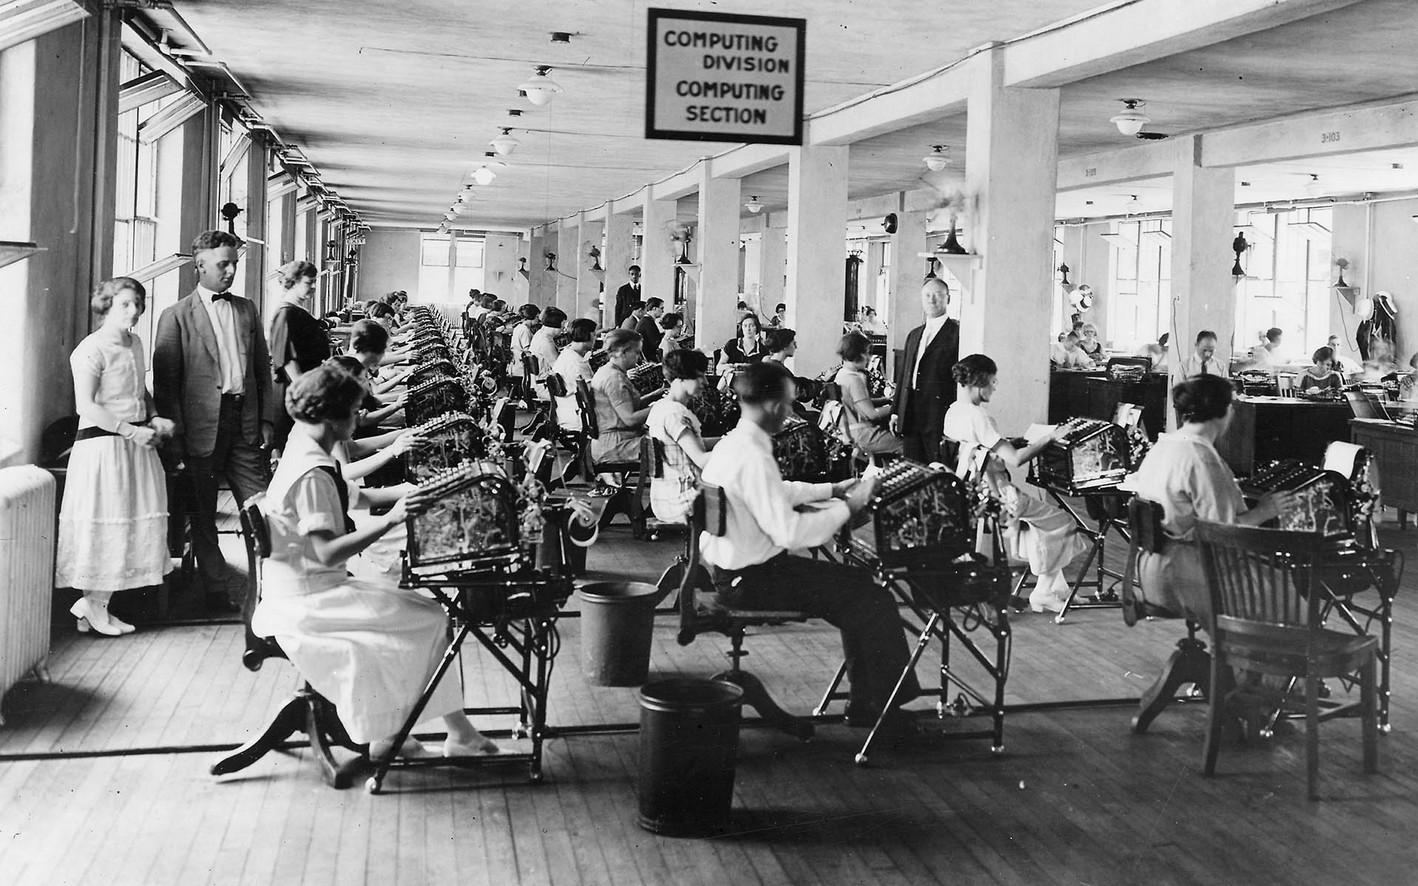
\includegraphics[scale=0.12]{pics/computers.png}
  \end{center}
\end{frame}


\begin{frame}[label=Program]
  \frametitle{Computer Programming}
  \framesubtitle{System status and bits}
  \begin{itemize}
   \item The status of the computer system is a string of \emph{bits}.
   \item A computer program is a sequence of instructions modifying 
       the status. The initial status is called the \emph{input}, the
          final state is the \emph{output} of the program.
   \item The instructions are bit patterns themselves, following
       conventions defined by the producer of the \emph{Processor},
       which translates operation codes into action on bits.
   \item All the information is registered in the computer using \emph{bits}.
  \end{itemize}
  \begin{center}
    
\includegraphics[scale=0.15]{pics/wand.png}
    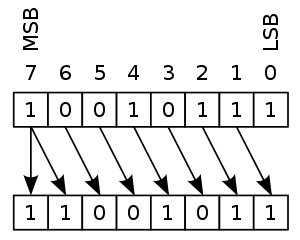
\includegraphics[scale=0.35]{pics/bits.png}
  \end{center}
\end{frame}


\begin{frame}[label=Coding]
  \frametitle{Information Coding}
  \framesubtitle{From letters to bit patterns}
  \begin{center}
    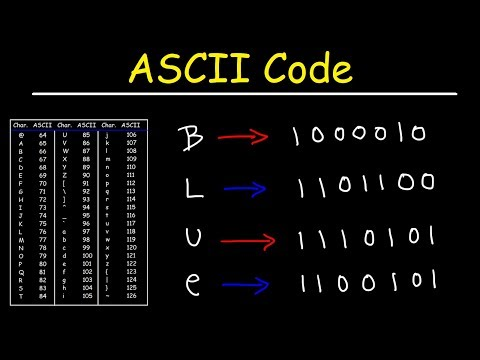
\includegraphics[scale=0.25]{pics/ascii.jpg}
  \end{center}
  \begin{itemize}
   \item The information is CODED : a $\rightarrow$ 01100001
   \item There are codes for
     \begin{itemize}
       \item Characters
       \item Exact Integer numbers
       \item Approximate representation of Real numbers
     \end{itemize}
   \item Special units in the processor can perform
     \begin{itemize}
       \item Character string manipulation
       \item Arithmetic operation
       \item Mathematical complex evaluation
     \end{itemize}
  \end{itemize}
\end{frame}


\begin{frame}[label=pdp11]
  \frametitle{The operating System}
  \framesubtitle{The origin of UNIX}
  \begin{columns}
    \begin{column}{0.50\textwidth}
      \begin{itemize}
        \item Hardware
      \begin{itemize}
        \item CPU, GPU, Motherboard, Cabling, Power
        \end{itemize}
        \item User
      \begin{itemize}
        \item Keyboard, Mouse, Monitor, etc
        \end{itemize}
        \item Software
      \begin{itemize}
        \item Application, Operating system
        \end{itemize}
      \end{itemize}
    \end{column}
    \begin{column}{0.50\textwidth}
      \begin{center}
        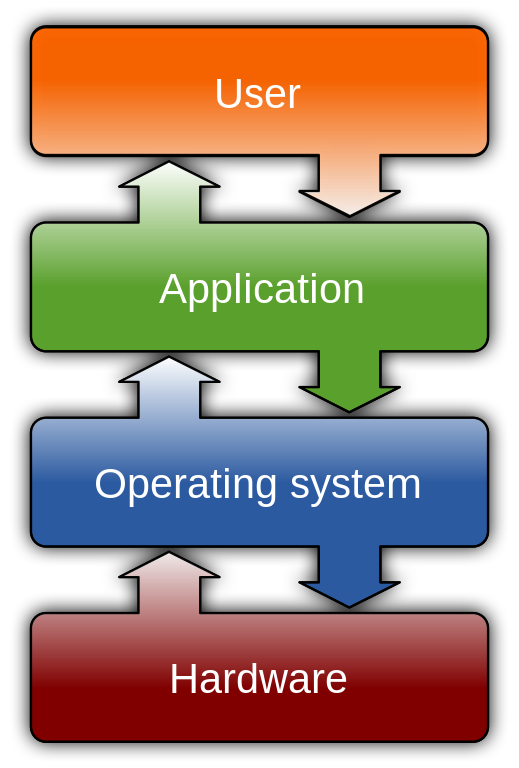
\includegraphics[scale=0.15]{pics/os.png}
      \end{center}
    \end{column}
  \end{columns}
  \begin{columns}
    \begin{column}{0.25\textwidth}
      \begin{center}
        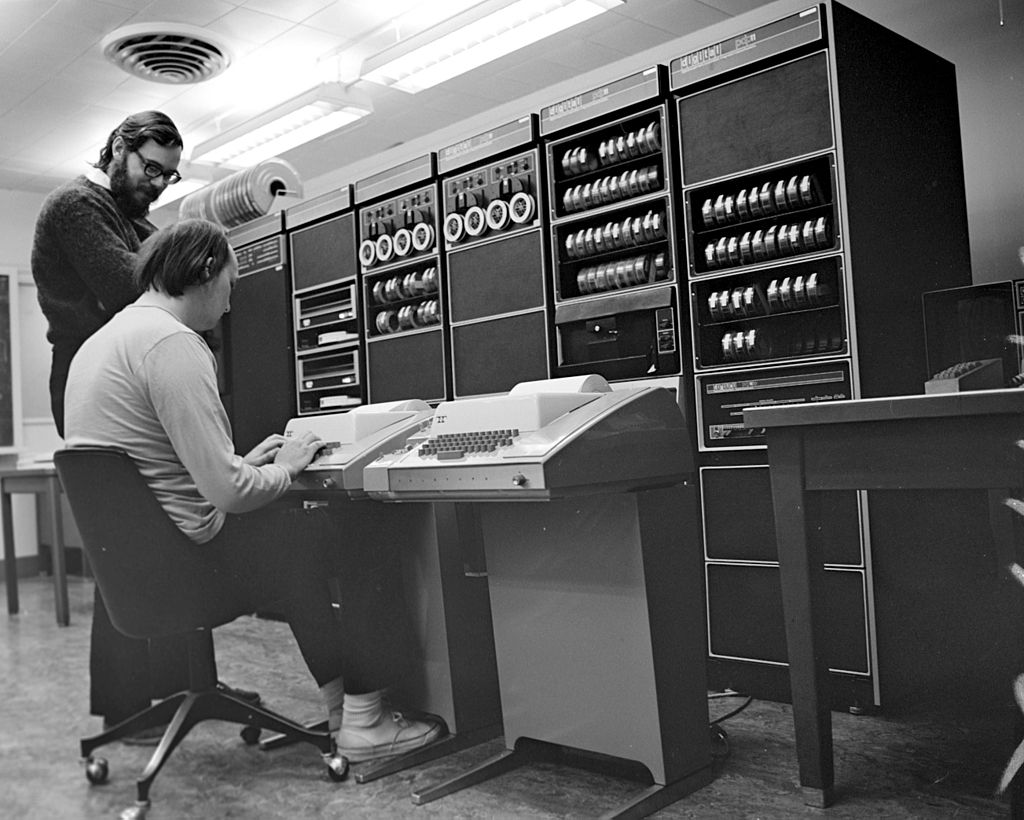
\includegraphics[scale=1.15]{pics/pdp11.jpg} \\
      \end{center}
    \end{column}
    \begin{column}{0.75\textwidth}
      \begin{itemize}
            \item 1969 - Multi-Tasking Multi-User Unix AT\&T
        \item 1991 - Free Unix OS for Intel X86 (Linux)
      \end{itemize}
    \end{column}
  \end{columns}
  \begin{flushleft}
    \tiny{By Peter Hamer: Ken Thompson (sitting) and Dennis Ritchie \\
          at PDP-11 Magnus Manske, CC BY-SA 2.0}
  \end{flushleft}
\end{frame}


\begin{frame}[label=unix]{UNIX Philosophy}
  \frametitle{The UNIX Philosophy}
  \framesubtitle{Why UNIX is such a good idea}
  \begin{enumerate}
    \item Make each program do one thing well. %To do a new job, build
      % afresh rather than complicate old programs by adding new "features".
    \item Expect the output of every program to become the input to another.
      %, as yet unknown, program. Don't clutter output with extraneous
      % information. Avoid stringently columnar or binary input formats.
      % Don't insist on interactive input.
    % \item Design and build software, even operating systems, to be tried
      % early, ideally within weeks. Don't hesitate to throw away the clumsy
      % parts and rebuild them.
    % \item Use tools in preference to unskilled help to lighten a programming
      % task, even if you have to detour to build the tools and expect to
      % throw some of them out after you've finished using them.
    % \item Write programs to handle text streams, because that is a
      % universal interface.
    \item Purpose of computation is data transformation
  \end{enumerate}
  \vfill
  \emph{$\dots$ at its heart is the idea that the power of a system comes
  more from the relationships among programs than from the programs themselves.
  Many UNIX programs do quite trivial things in isolation, but, combined with
  other programs, become general and useful tools. \dots}
  \newline
  \begin{flushright}
  \tiny{The UNIX Programming Environment, Brian Kernighan and Rob Pike, 1984}
  \end{flushright}
\end{frame}


\begin{frame}[label=os]
  \frametitle{The Linux Revolution}
  \framesubtitle{Why a free OS is a good idea}
  \begin{center}
    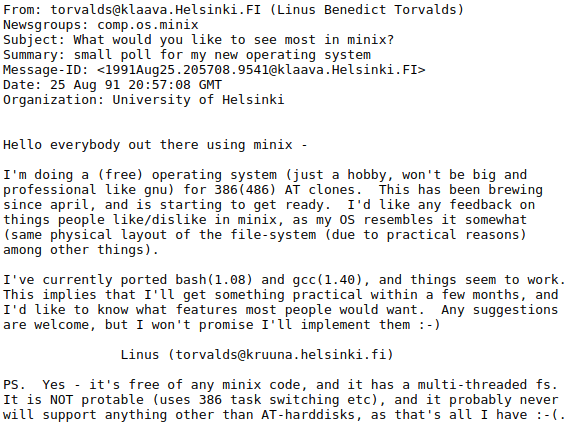
\includegraphics[scale=0.5]{pics/linux-first-announcement-email.png}
  \end{center}
\end{frame}


\begin{frame}[label=gnu]
  \frametitle{The Free Software Movement}
  \framesubtitle{Free Software as in Freedom}
  \begin{columns}[T]
    \begin{column}{.68\textwidth}
      \begin{block}{The Freedom to}
        \begin{itemize}
          \item run the program as you wish, for any purpose
          \item study how the program works, and change it as you wish
          \item redistribute copies so you can help others
          \item distribute copies of your modified versions to others
        \end{itemize}
      \end{block}
    \end{column}
    \hfill
    \begin{column}{.32\textwidth}
      \begin{flushright}
        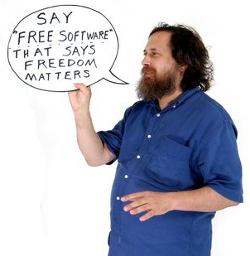
\includegraphics[scale=0.35]{pics/rms1.png} \\
      \end{flushright}
    \end{column}
  \end{columns}
  \begin{center}
    
\includegraphics[scale=0.25]{pics/GPL.png}
  \end{center}
\end{frame}


\begin{frame}[label=architecture]
  \frametitle{Linux architecture}
  \framesubtitle{Linux is the kernel and we do not hate it!}
  \begin{columns}[T]
    \begin{column}{.23\textwidth}
      \vspace{7mm}
      
\includegraphics[scale=0.5]{pics/UNIX-HATERS_Handbook_cover_ISBN_1-56884-203-1.png}
    \end{column}
    \begin{column}{.73\textwidth}
      \begin{itemize}
      \item The Linux kernel is a program that loads all the other programs and
        supervise the resources allocated to each one of them, providing
        locking and I/O services.
      \item The system services \emph{(daemons)} are programs running on the
        system and providing facilities that allow or enhance access to system
        resources.
      \item User programs are controlled interactively or through batch job
        submission system by physical users concurrently accessing system
        resources through a multi tasking sharing of the CPU(s).
    \end{itemize}
    \end{column}
  \end{columns}
\end{frame}


\begin{frame}[label=linux]
  \frametitle{Install Linux OS}
  \framesubtitle{A Linux Distribution}
  \begin{center}
    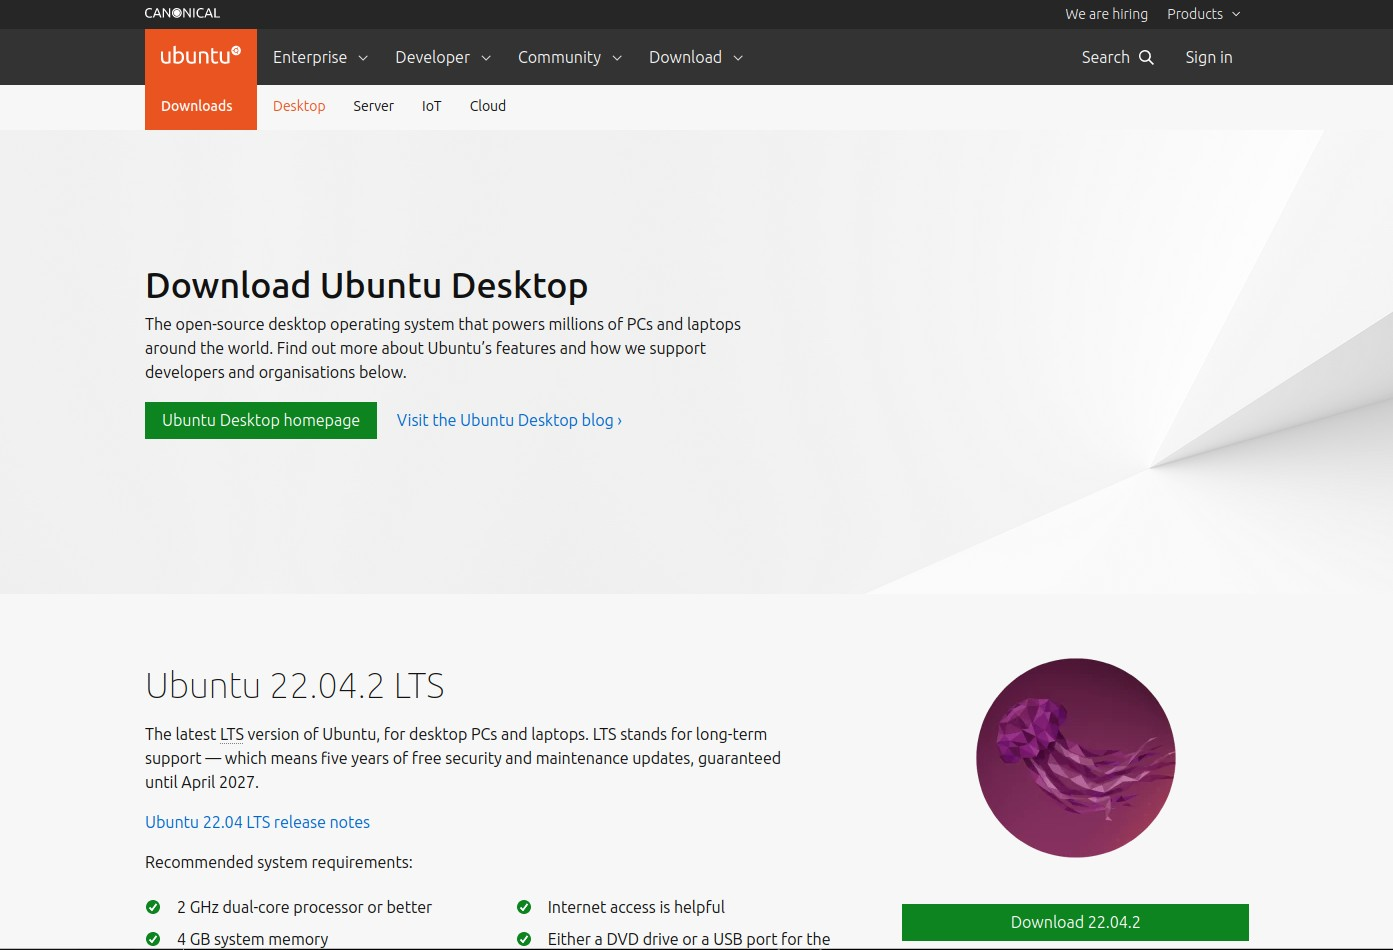
\includegraphics[scale=0.25]{pics/ubuntu.png}
  \end{center}
\end{frame}


\begin{frame}[label=macos]
  \frametitle{Install Free Software on MacOS}
  \framesubtitle{HomeBrew}
  \begin{center}
    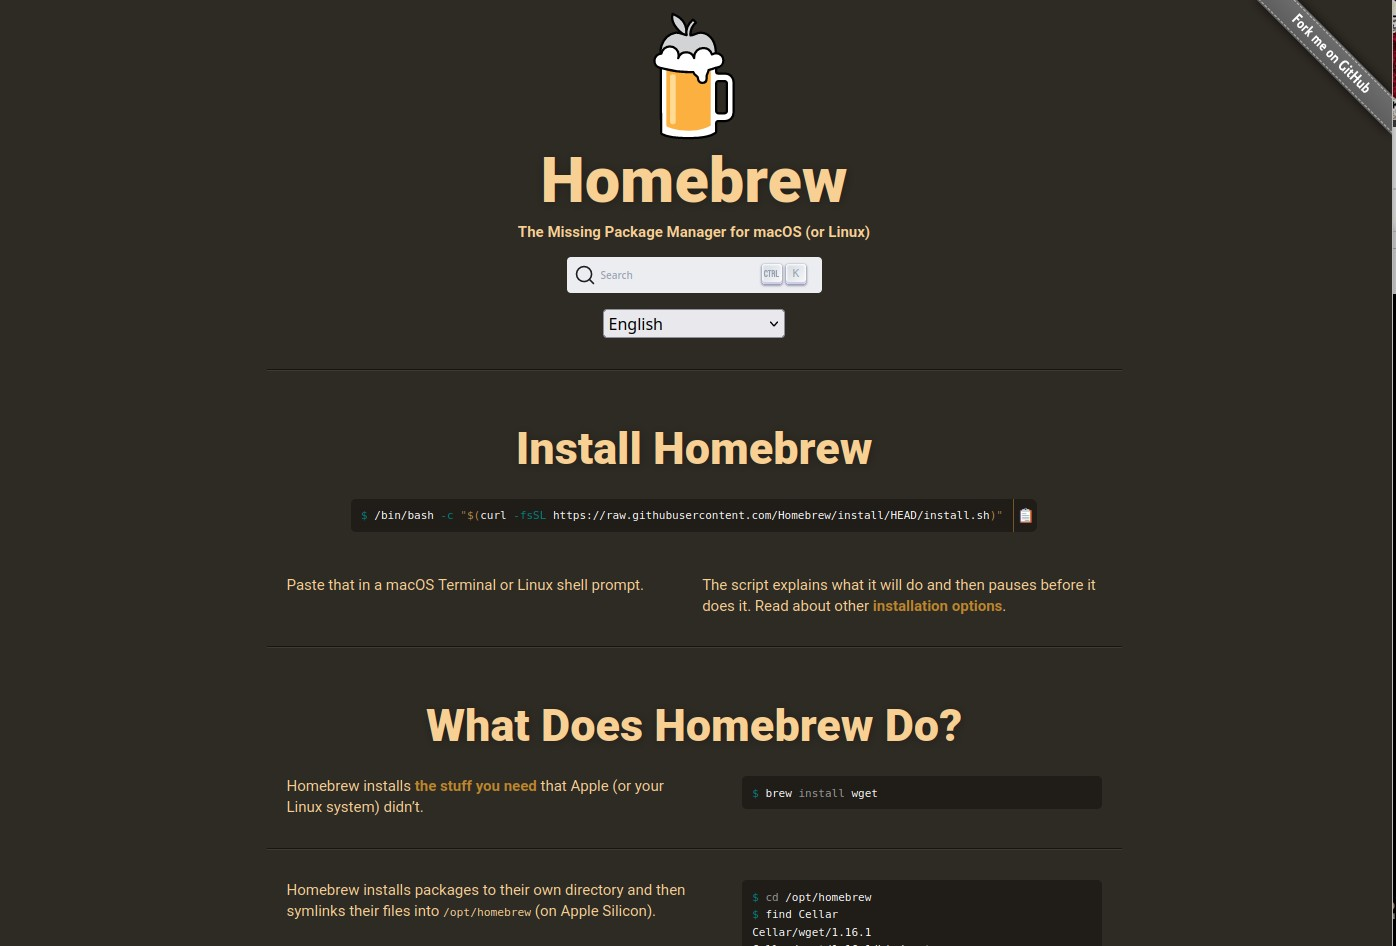
\includegraphics[scale=0.25]{pics/brew.png}
  \end{center}
\end{frame}


\begin{frame}[label=windows]
  \frametitle{Install Free Software on Windows}
  \framesubtitle{WSL - Windows Subsystem for Linux}
  \begin{center}
    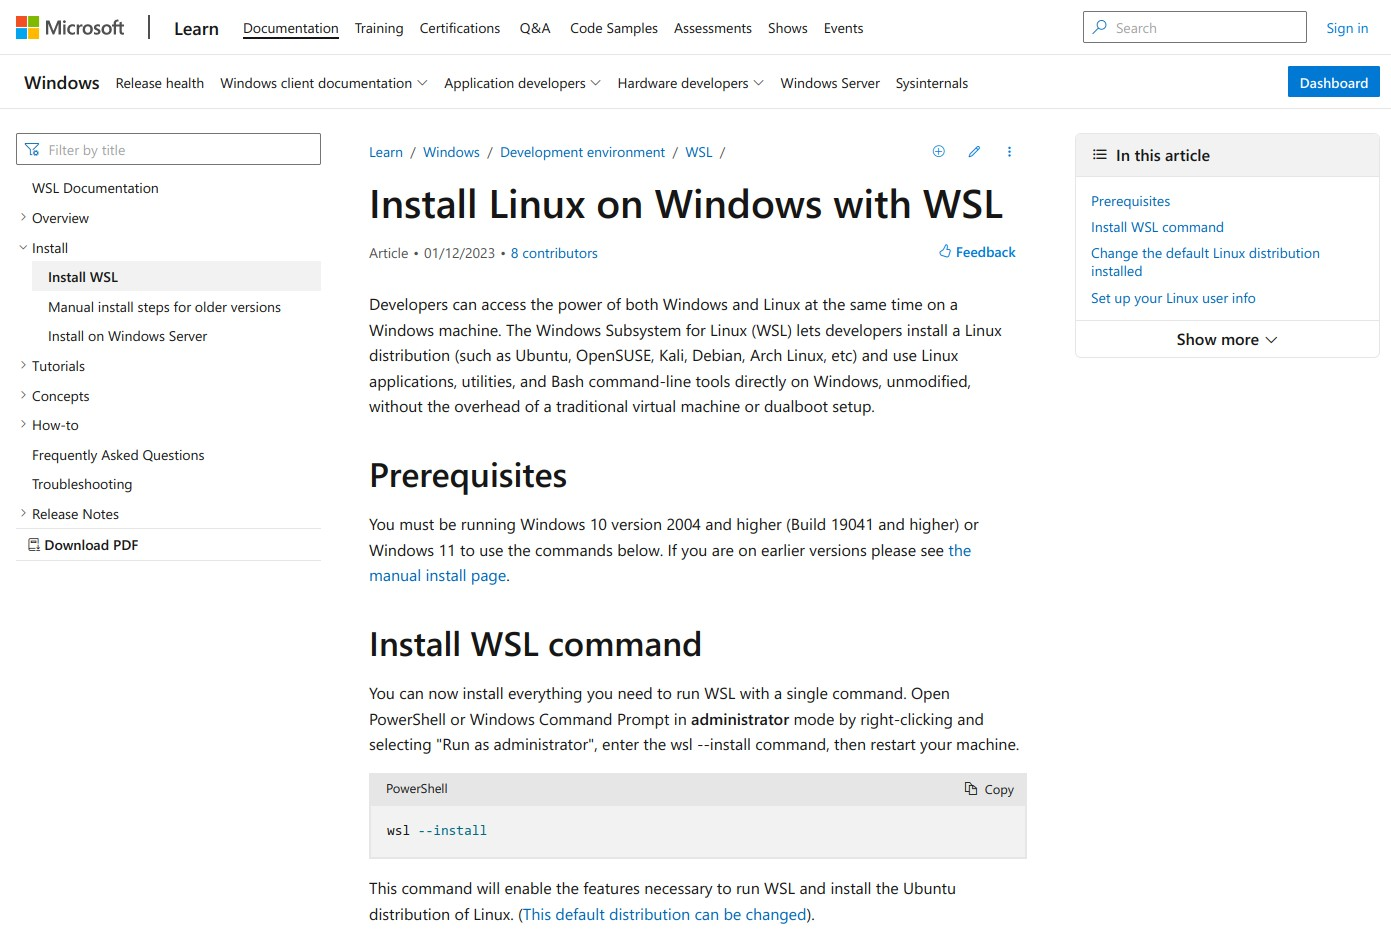
\includegraphics[scale=0.25]{pics/WSL.png}
  \end{center}
\end{frame}


\begin{frame}[label=install]
  \frametitle{Install Linux}
  \framesubtitle{Let's try install}
  \begin{center}
    
\includegraphics[scale=0.11]{pics/TUX_G2.svg.png}
  \end{center}
\end{frame}


\end{document}

%vim: tabstop=8 expandtab shiftwidth=2 softtabstop=2 spell spelllang=en_GB
